\label{sec::real-time}
\subsection{Device under Test}
\label{sec::experiment}
\todo[inline]{Replace this section with Berdina}
Though experiments and designs are constantly evolving, at the core of this group's research is an \gls{set} used to perform electron spin readout. The apparatus I am applying my work to is by no means comprehensive, but it serves as a reference point in a proven device \cite{morello2010single}. To improve spin initialisation with this particular device would therefore be extensible to other devices and experiments.
Figure \ref{fig::thesis_experiment} shows a general layout used to control and read from an \gls{set}.

\begin{figure}[htbp!]
	\centering
	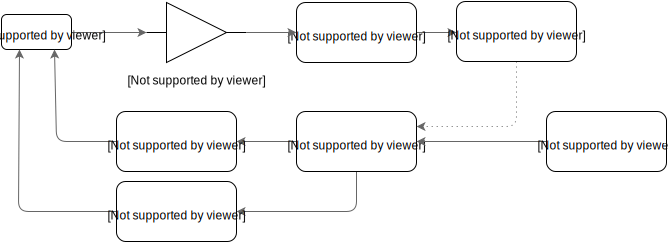
\includegraphics[width=\textwidth]{thesis_experiment.pdf}
	\caption{Block diagram of experiment}
	\label{fig::thesis_experiment}
\end{figure}


Figure \ref{fig::set_layout} shows the physical device that will be similar to one I will be testing my solution on. This devices has various voltage-controlled nodes, such as the top gate to induce a layer of electrons on the boundary, the left and right barriers to remove this layer, forming tunnel junctions to the island, and finally the plunger which can act at the gate as defined in section \ref{sec::set}.

\begin{figure}[htbp!]
	\centering
	\includegraphics[width=\textwidth]{set_layout}
	\caption[Layout of an \gls{set}]{The layout of an \gls{set}\cite{morello2010single}}
	\label{fig::set_layout}
\end{figure}

\subsection{Set-Up and Equipment}
	\todo[inline]{perhaps explain here about the dilution refrigerator and the millikelvin environment}

\subsection{Process}

	\subsubsection{Gate Stimulus, NMR and ESR}
		To allow for precise control and measurement of the steering time applied to the electron donor, an electrostatic environment needed to be defined, along with radio and microwave stimulus. The \gls{set} donor is coupled capacitively to a number of gates, and so the tunnelling of an electron can be controlled simply by shifting the degenerate electron energy level about the Fermi level of the island. Once a magnetic field is applied, the degenerate electron energy levels split between the higher energy spin-up state, and the lower energy spin-down state. When tuned to the correct gate voltages, a spin-down electron's energy will be below the Fermi level, while a spin-up electron's energy will be above the Fermi energy, allowing tunnelling to unoccupied states. This is the ideal voltage to set our initialisation and readout levels. In Figure \ref{fig::sequence}, the \gls{set} control gate is being changed throughout the experiment, from empty to initialisation, then followed by a sequence of plunges and readouts. The plunge voltage will take the donor electron below the Fermi level, and so neither spin-state will be able to tunnel, as there are no available states in the reservoir, assuming the device is near absolute zero.
		
		
		\begin{figure}[htbp!]
			\centering
			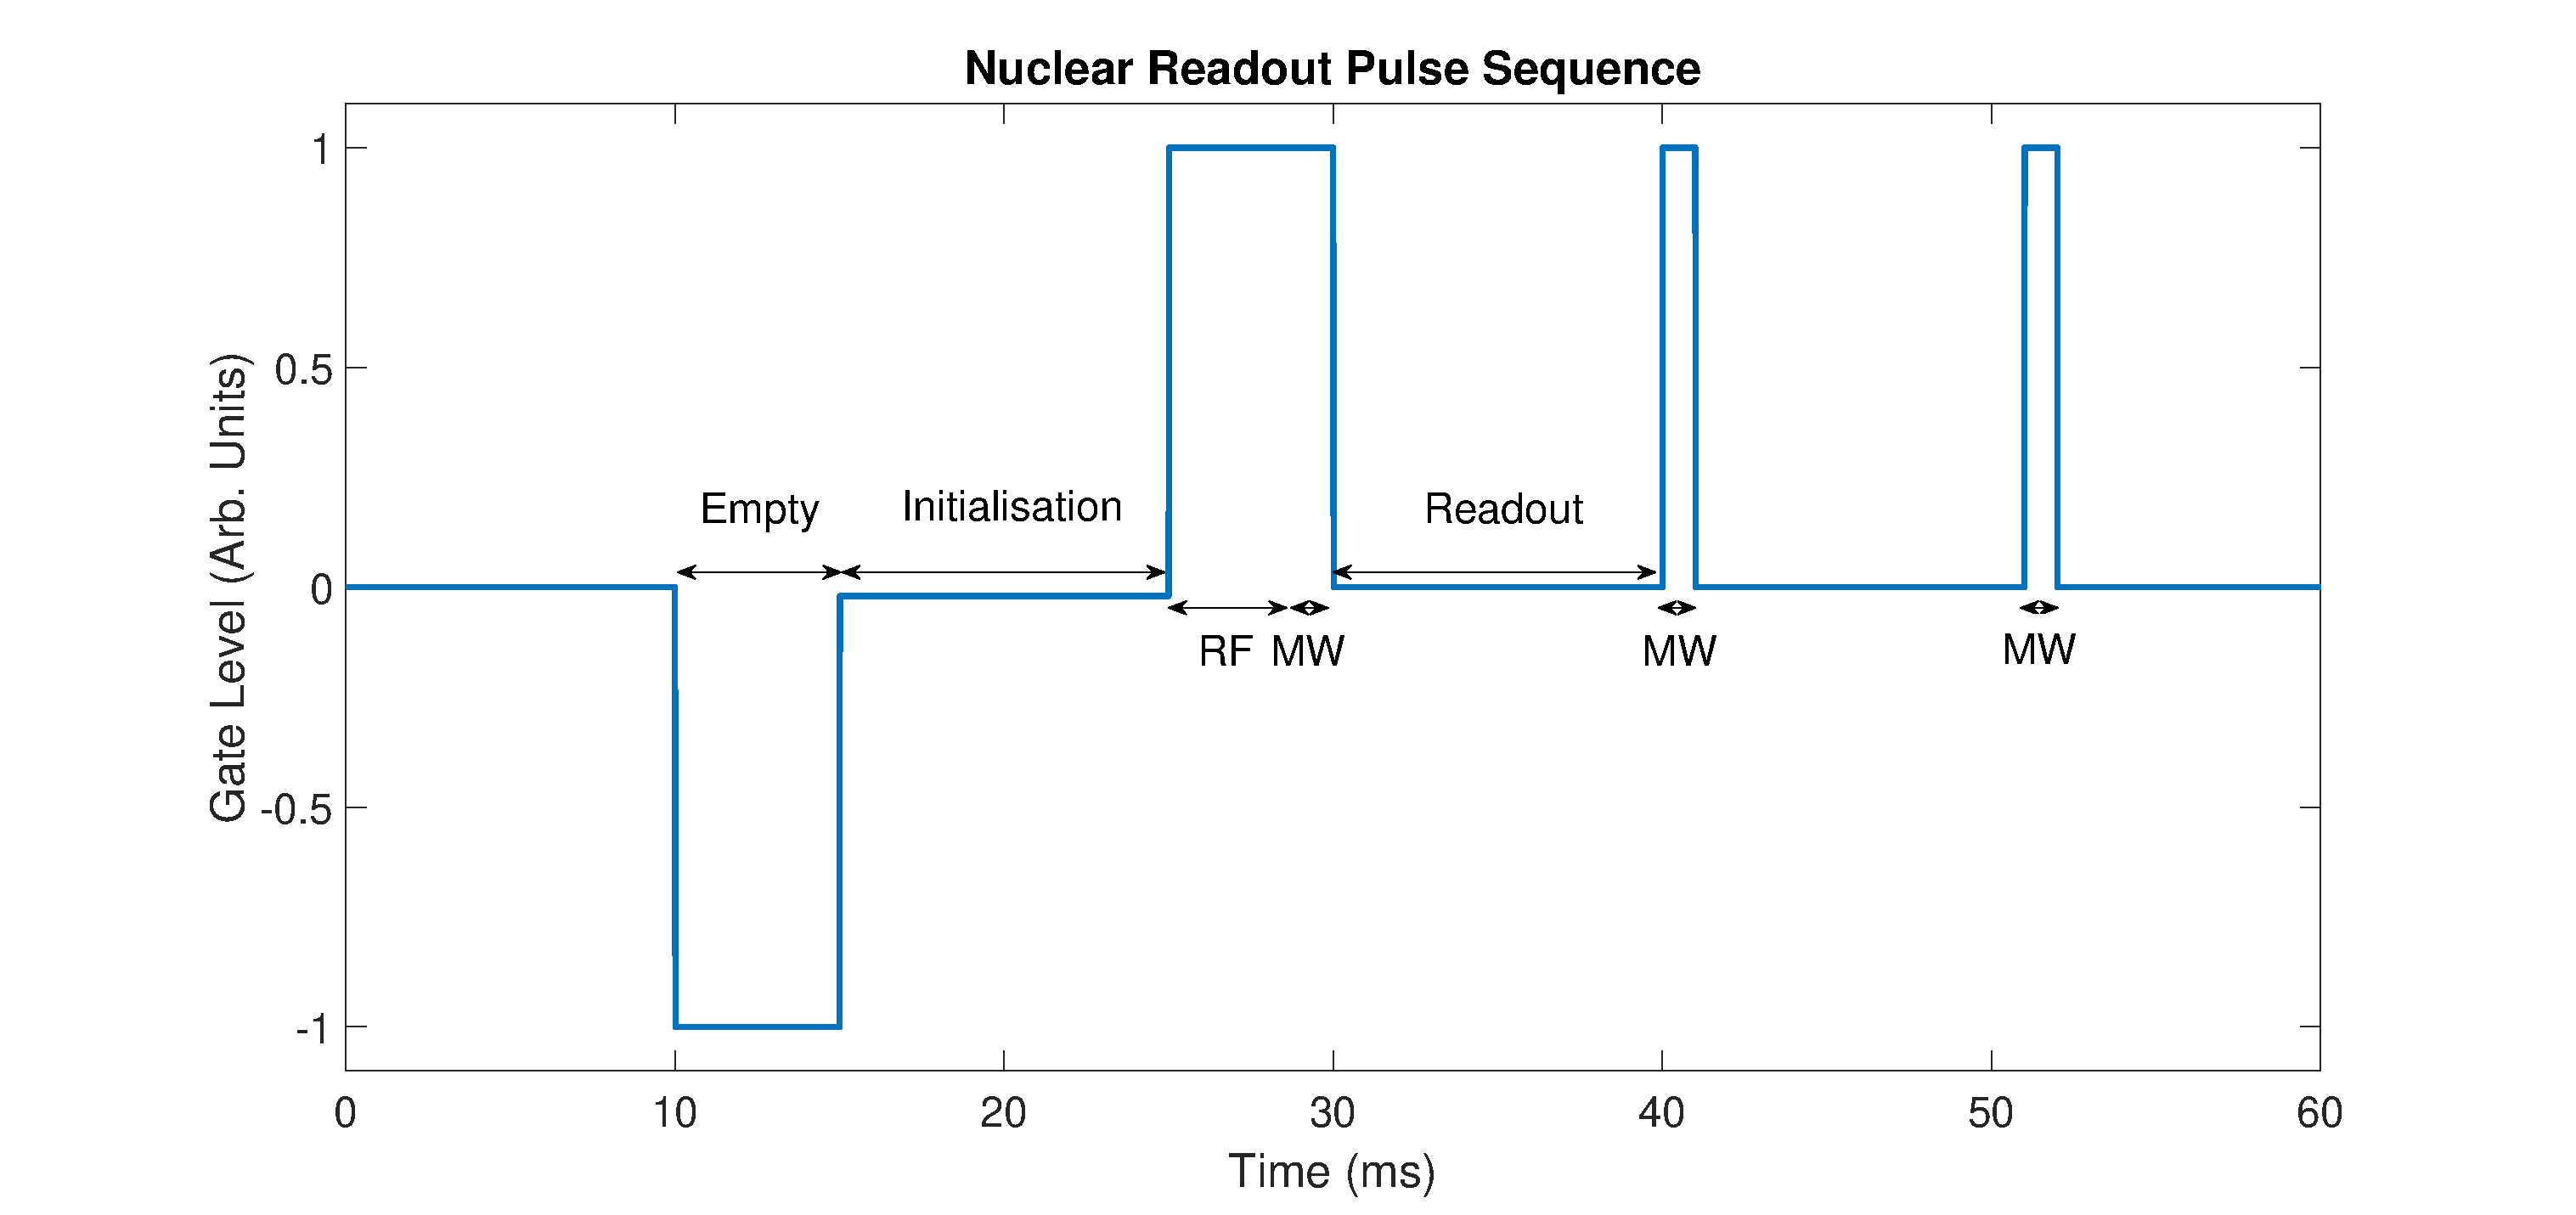
\includegraphics[width=\textwidth]{sequenceFigure}
			\caption{The control sequence, describing both gate levels as well as \gls{rf} and \gls{mw} stimulus, applied for this experiment.}
			\label{fig::sequence}
		\end{figure}
		
		During the initial plunge, a \gls{rf} pulse and a \gls{mw} pulse will be applied, to map the state of the donor electron to the nucleus and then to map the state of the nucleus to the electron, respectively. Mapping from nucleus to electron place during this stage is a short-hand method of beginning the readout phase, without first returning to the readout level.
		
		These \gls{rf} and \gls{mw} pulses are applying \gls{nmr} and \gls{esr}, conditional upon the state of the electron, for \gls{nmr}, and conditional on the state of the nucleus, for \gls{esr}. This is best explained by Figure \ref{fig::spin_levels}, where the state transitions are shown to require distinct driving frequencies, $\nu_{e1}, \nu_{e2}, \nu_{n1} \textrm{ and } \nu_{n2}$. Since the electron spin is expected to be spin-down when the \gls{rf} pulse is performed, the driving frequency to perform \gls{nmr} will be $\nu_{n2}$. Using this method we will perform a $\pi$-pulse, which will flip the nucleus state from spin-up to spin-down, or vice versa given that is in initially in one of these states. For each consecutive readout, the nucleus is expected to flip, as ideally each time a spin-down electron is loaded followed by a successful $\pi$-pulse.
		
		Once the nuclear state has been prepared, the sequence of electron state mapping and readout commences, which performs \gls{esr} conditional upon the state of the nucleus. The driving frequency for this transition is $\nu_{e2}$, so the readout phases should show tunnel events if the nucleus is spin-up.
	
		This measurement is repeated 20 times, to determine the state of the nucleus accurately, and then the experiment is repeated a set number of times (for the data presented in this report, the nuclear readout was performed between 500 and 2000 times). 
		
	\subsubsection{Magnetic Field Variation}
		Once the characteristics of quantum steering are established at a set magnetic field, it will be worthwhile studying the impact of this approach at lower magnetic fields. Lower magnetic fields incur more initialisation errors due to a smaller Zeeman splitting than with a higher magnetic field. If there is little affect on the efficacy of quantum steering for initialisation, and also on the readout fidelity, then a spin device can become far more practicable, as the level of \gls{esr} control is much simpler at lower driving frequencies, and often there are simply more numerous devices available at lower frequencies. The primary fields of consideration are 1.4 T, 1.0 T, and 0.7 T, which correspond to \gls{esr} frequencies  $\nu_{e1}, \nu_{e2} \approx$ 39 GHz, 28 GHz and 20 GHz, respectively.
		
		Furthermore, once the magnetic field on the Z-axis is below 1.0 T, we are able to define a full 3-dimensional magnetic environment using 2-dimensional vector magnets in the XY-plane, perpendicular to the large magnetic field described above. 1.0 T is the limit of these vector magnets, and as such full 3-dimensional control is impossible above this threshold.
		\todo{tie this together nicely...}
		
	